% PREAMBLE
\documentclass[11pt]{amsart}
\usepackage[T1]{fontenc}
\usepackage{lmodern}
\usepackage{microtype}
\usepackage{amsmath,amssymb}
\usepackage{mathtools}
\usepackage{graphicx}
\usepackage{booktabs}
\usepackage{tikz}
\usepackage[colorlinks=true,linkcolor=blue!45!black,citecolor=blue!45!black,urlcolor=blue!45!black]{hyperref}
\usepackage[capitalize]{cleveref}

\newtheorem{theorem}{Theorem}[section]
\newtheorem{proposition}[theorem]{Proposition}
\newtheorem{lemma}[theorem]{Lemma}
\newtheorem{corollary}[theorem]{Corollary}
\newtheorem{conjecture}[theorem]{Conjecture}
\theoremstyle{definition}
\newtheorem{definition}[theorem]{Definition}
\newtheorem{fact}[theorem]{Fact}
\theoremstyle{remark}
\newtheorem{remark}[theorem]{Remark}

\title{Pairwise Coprimality in the Menger Sponge}
\author{Carlo Mitchener}
\email{carlo.mitchener@gmail.com}
\date{2026-08-23}

% PAPER
\begin{document}

\begin{abstract}
Drilling the holes of the Menger sponge costs its corner coordinates exactly twelve and a quarter percent of their odds of sharing no prime factor in pairs. We prove that the fraction of level-$L$ sponge points $(x,y,z)$ whose three coordinates are pairwise coprime converges, as $L\to\infty$, to $\tfrac{13}{20}\prod_{p\ne3}(1-3p^{-2}+2p^{-3})=0.251620868\ldots$, which is exactly $\tfrac{351}{400}$ of the classical three-integer pairwise-coprimality constant. The proof is a general one: for any digit design $F\subseteq\{0,\dots,q-1\}^3$ in a prime base $q$ whose difference set generates $\mathbb Z^3$, the same density formula holds as soon as $|F|>q\kappa_I$ for each of the three coordinate pairs $I$, where $\kappa_I$ is the largest fibre of the restriction of $F$ to $I$. The sponge clears this bar because a pair-fibre has three elements and $20>3\cdot3$; a single coordinate has an eight-element fibre and would not. The six levels we can count exactly all sit below the constant, and we identify the leading cause: the sponge digits are biased modulo $2$, which conjecturally sets a geometric approach rate.
\end{abstract}

\maketitle

\begin{figure}[!ht]
\centering
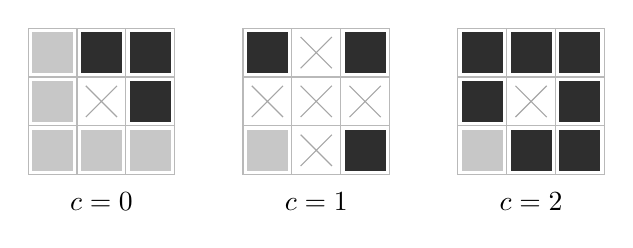
\begin{tikzpicture}[scale=0.62]
\foreach \s/\lab in {0/{$c=0$}, 1/{$c=1$}, 2/{$c=2$}}{
  \begin{scope}[xshift=\s*4.4cm]
    \draw[gray!55] (0,0) grid (3,3);
    \node at (1.5,-0.55) {\lab};
  \end{scope}
}
\foreach \a/\b in {1/2,2/1,2/2}{\fill[black!82] (\a+0.08,\b+0.08) rectangle (\a+0.92,\b+0.92);}
\foreach \a/\b in {0/0,0/1,0/2,1/0,2/0}{\fill[black!22] (\a+0.08,\b+0.08) rectangle (\a+0.92,\b+0.92);}
\foreach \a/\b in {1/1}{\draw[gray!70] (\a+0.18,\b+0.18) -- (\a+0.82,\b+0.82) (\a+0.18,\b+0.82) -- (\a+0.82,\b+0.18);}
\begin{scope}[xshift=4.4cm]
\foreach \a/\b in {0/2,2/0,2/2}{\fill[black!82] (\a+0.08,\b+0.08) rectangle (\a+0.92,\b+0.92);}
\foreach \a/\b in {0/0}{\fill[black!22] (\a+0.08,\b+0.08) rectangle (\a+0.92,\b+0.92);}
\foreach \a/\b in {0/1,1/0,1/1,1/2,2/1}{\draw[gray!70] (\a+0.18,\b+0.18) -- (\a+0.82,\b+0.82) (\a+0.18,\b+0.82) -- (\a+0.82,\b+0.18);}
\end{scope}
\begin{scope}[xshift=8.8cm]
\foreach \a/\b in {0/1,0/2,1/0,1/2,2/0,2/1,2/2}{\fill[black!82] (\a+0.08,\b+0.08) rectangle (\a+0.92,\b+0.92);}
\foreach \a/\b in {0/0}{\fill[black!22] (\a+0.08,\b+0.08) rectangle (\a+0.92,\b+0.92);}
\foreach \a/\b in {1/1}{\draw[gray!70] (\a+0.18,\b+0.18) -- (\a+0.82,\b+0.82) (\a+0.18,\b+0.82) -- (\a+0.82,\b+0.18);}
\end{scope}
\end{tikzpicture}
\caption{The twenty-seven digit vectors $(a,b,c)$, drawn as three $3\times3$ slices. Seven are crossed out: they have two or more digits equal to $1$ and the sponge deletes them. Of the twenty survivors, the thirteen dark ones have at most one digit equal to $0$; the seven pale ones have two or more zeros, and a point whose last digit vector is pale has two coordinates divisible by $3$. The ratio $13/20$ is the whole effect of the base prime, at every level.}
\label{fig:design}
\end{figure}

\section{Introduction}
\label{sec:intro}

Take a cube, cut it into twenty-seven equal subcubes, remove the seven that touch the centre, and repeat forever inside each of the twenty survivors. That is the Menger sponge. Address a survivor at level $L$ by its $L$ base-three digit vectors: each digit vector is a triple $(a,b,c)$ of digits in $\{0,1,2\}$, a digit equal to $1$ meaning ``middle slab in this direction'', and a subcube survives exactly when at most one of its three digits is a $1$. \Cref{fig:design} shows the twenty survivors. Reading the three coordinate digit strings as integers turns the level-$L$ sponge into a set $S_L$ of $20^L$ integer points.

Now ask an arithmetic question about a geometric object. Pick a sponge point at random. How often are its three coordinates pairwise coprime, that is, how often do no two of them share a prime factor?

For three integers drawn at random from a long interval the answer is a classical constant, computed by T\'oth~\cite{toth}:
\[
C_3=\prod_p\Bigl(1-\frac{3}{p^2}+\frac{2}{p^3}\Bigr)
=\prod_p\Bigl(1-\frac1p\Bigr)^2\Bigl(1+\frac2p\Bigr)
=0.2867474284\ldots,
\]
recorded as \href{https://oeis.org/A065473}{A065473}~\cite{oeisA065473}. The sponge is a thin, self-similar subset of the lattice, so there is no reason for it to inherit that number, and it does not. It gets a different one, and the difference is confined to a single prime.

\begin{quote}
\textbf{Answer.} The limiting fraction is $\frac{13}{20}\prod_{p\ne3}(1-3p^{-2}+2p^{-3})=0.2516208684\ldots$, which is $\frac{351}{400}C_3$. Every prime except $3$ behaves as it does on the full lattice. At $p=3$ the lattice factor $20/27$ is replaced by $13/20$, and that one swap costs the sponge exactly $\frac{49}{400}=12.25\%$ of its pairwise-coprimality odds.
\end{quote}

The number $13/20$ is visible in \cref{fig:design} and needs no analysis. A coordinate is divisible by $3$ exactly when its last base-three digit is $0$, so a point has two coordinates divisible by $3$ exactly when its last digit vector has two or more zeros. Seven of the twenty digit vectors are like that; thirteen are not. Nothing about the higher digits enters, so the fraction is exactly $13/20$ at every level, not merely in the limit.

The work is in the other primes. A prime $p\ne3$ cannot read a single digit; it sees the whole number, and one must prove that the sponge's coordinates spread out evenly modulo $p$ and that no conspiracy hides among the very large primes. The first is a character estimate. The second is a counting bound with a twist we make the centrepiece: instead of asking how many sponge points have a fixed coordinate divisible by $m$, we ask how many have two prescribed coordinates divisible by $m$, and we count the digit strings by fibring the design over that pair of coordinates. The gain is decisive. Fibring over one coordinate leaves fibres of size $8$ and an exponent $\log_3(20/8)=0.83<1$, which proves nothing; fibring over a pair leaves fibres of size $3$ and an exponent
\[
\alpha=\log_3\frac{20}{3}=1.7268\ldots>1,
\]
and an exponent above $1$ closes the tail. This is the general criterion of \cref{thm:general}: a base-$q$ design with $k$ digit vectors settles the pairwise question as soon as $k>q\kappa_I$ for each coordinate pair. The sponge satisfies $20>3\cdot3$ with room to spare.

One honest warning belongs on page one, because the finite-level counts look at first like a refutation. An exact census of all $64$ million level-six points gives a pairwise-coprime fraction of $0.2365826\ldots$, six percent \emph{below} the limit, and the six values available climb towards the constant from underneath rather slowly. \Cref{sec:results} explains why, exactly: the sponge's digits are biased modulo $2$. A single coordinate is odd with probability $1/5$ per digit, so it is even with probability $\frac12(1+(3/5)^L)$ rather than $\frac12$, and the level-$L$ local factor at $p=2$ is
\[
\beta_L=\frac12-\frac34\Bigl(\frac35\Bigr)^{L}+\frac14\Bigl(-\frac15\Bigr)^{L},
\]
which is $0.4416$ at $L=5$ against its limit $0.5$. That one factor accounts for the whole visible deficit and slightly overshoots it. We conjecture on that evidence, in \cref{con:rate}, that the approach is geometric with ratio $3/5$; if it is, the deficit is small only when $(3/5)^L$ is, and at $L=6$ that is still $0.047$.

The paper is organised as the shelf requires: \cref{sec:def} fixes the objects, \cref{sec:results} states everything, \cref{sec:proofs} proves it, \cref{sec:repro} says how to re-run every number.

\section{Definitions}
\label{sec:def}

\begin{definition}[The design and the point set]
\label{def:sponge}
Let
\[
F=\bigl\{(a,b,c)\in\{0,1,2\}^3:\ \text{at most one of }a,b,c\text{ equals }1\bigr\},
\qquad |F|=20 .
\]
For $L\ge0$ let
\[
S_L=\Bigl\{\ \Bigl(\sum_{j=0}^{L-1}a_j3^j,\ \sum_{j=0}^{L-1}b_j3^j,\ \sum_{j=0}^{L-1}c_j3^j\Bigr)\ :\ (a_j,b_j,c_j)\in F\ \text{for all }j\ \Bigr\},
\]
counted with multiplicity of digit strings, so that $|S_L|=20^L$. Points are always sampled uniformly over digit strings. Write
\[
P_L=\frac{1}{20^L}\#\bigl\{(x,y,z)\in S_L:\gcd(x,y)=\gcd(x,z)=\gcd(y,z)=1\bigr\}.
\]
\end{definition}

Distinct digit strings give distinct points, since base-three expansion is unique, so the multiplicity remark only fixes the sampling measure.

\begin{definition}[Coprimality convention]
\label{def:gcd}
We use $\gcd(0,n)=n$, hence $\gcd(0,1)=1$, so that in principle a point with a zero coordinate could be pairwise coprime. For this design none is, at any level. Suppose $x_1=0$. Pairwise coprimality then forces $\gcd(x_1,x_2)=x_2=1$ and $\gcd(x_1,x_3)=x_3=1$, so the last digit vector of the point is $(0,1,1)$, which has two entries equal to $1$ and is therefore not in $F$. The same argument applies to the other two coordinates. Hence no point counted by $P_L$ has a zero coordinate and the census is the same under either convention, even though zero coordinates are not rare: $x_1=0$ holds for a $(2/5)^L$ fraction of $S_L$, since eight of the twenty digit vectors have first entry $0$.
\end{definition}

\begin{definition}[General digit designs, fibres, exponent]
\label{def:general}
Let $q$ be a prime and let $F\subseteq\{0,\dots,q-1\}^3$ with $k=|F|\ge2$. Define $S_L(F)$ and $P_L(F)$ exactly as in \cref{def:sponge} with $q$ in place of $3$ and $F$ in place of the sponge design. For a set of coordinates $I\subseteq\{1,2,3\}$ let $v|_I$ denote the restriction of $v\in F$ to the coordinates in $I$ and put
\[
\kappa_I=\max_{w}\#\{v\in F:\ v|_I=w\},
\qquad
\alpha_I=\log_q\frac{k}{\kappa_I}.
\]
Say that $F$ is \emph{spanning} if the differences $\{v-v':v,v'\in F\}$ generate $\mathbb Z^3$ as a group.
\end{definition}

For the sponge design, direct enumeration of the twenty vectors gives $\kappa_I=3$ for each of the three pairs $I$ and $\kappa_{\{i\}}=8$ for each single coordinate, so
\[
\alpha=\alpha_{\text{pair}}=\log_3\frac{20}{3}=1.726833\ldots,
\qquad
\alpha_{\text{single}}=\log_3\frac{20}{8}=0.834\ldots.
\]
The sponge design is spanning: $(0,0,0)$ and the three unit vectors all lie in $F$.

\section{Results}
\label{sec:results}

\begin{theorem}[The sponge density]
\label{thm:sponge}
With $P_L$ as in \cref{def:sponge},
\[
\lim_{L\to\infty}P_L
=\frac{13}{20}\prod_{p\ne3}\Bigl(1-\frac{3}{p^2}+\frac{2}{p^3}\Bigr)
=\frac{351}{400}\,C_3
=0.251620868451255\ldots,
\]
where $C_3=\prod_p(1-3p^{-2}+2p^{-3})=0.286747428434479\ldots$ is the classical three-integer pairwise-coprimality constant of \emph{\cite{toth,oeisA065473}}.
\end{theorem}

\begin{theorem}[Any digit design that clears the bar]
\label{thm:general}
Let $q$ be a prime and $F\subseteq\{0,\dots,q-1\}^3$ a design with $k=|F|$ that is spanning in the sense of \cref{def:general} and satisfies
\[
k>q\,\kappa_I\qquad\text{for each of the three coordinate pairs } I\subseteq\{1,2,3\},
\]
equivalently $\alpha_I>1$ for each pair. Then
\[
\lim_{L\to\infty}P_L(F)
=\delta_q(F)\prod_{p\ne q}\Bigl(1-\frac{3}{p^2}+\frac{2}{p^3}\Bigr),
\]
where
\[
\delta_q(F)=\frac{1}{k}\#\{v\in F:\text{at most one entry of }v\text{ is }0\}.
\]
Moreover $\delta_q(F)$ is the exact fraction of $S_L(F)$ with no coordinate pair divisible by $q$, for every $L\ge1$.
\end{theorem}

\Cref{thm:sponge} is the case $q=3$, $k=20$, $\kappa_{\text{pair}}=3$, $\delta_3=13/20$; the hypothesis reads $20>9$. Both hypotheses do work. Spanning is what makes the residues equidistribute, and without it the conclusion can fail while the pair condition holds: take $q=7$ and let $F$ be the $196$ vectors whose first entry is even: then $\kappa_I\le7$ for every pair and $196>7\kappa_I$, but every point has an even first coordinate, the residue vector modulo $2$ is not uniform, and the true density is smaller than the formula. The pair condition is what the tail estimate consumes, and it is not decorative: see \cref{rem:fibre}.

\begin{proposition}[The base prime is exact at every level]
\label{prop:base}
For every $L\ge1$, the fraction of points of $S_L$ having no two coordinates divisible by $3$ is exactly $13/20$.
\end{proposition}

\begin{proposition}[The bias at two, in closed form]
\label{prop:two}
For every $L\ge0$, the fraction of points of $S_L$ having at most one even coordinate is exactly
\[
\beta_L=\frac12-\frac34\Bigl(\frac35\Bigr)^{L}+\frac14\Bigl(-\frac15\Bigr)^{L},
\]
and a single coordinate is even with probability exactly $\tfrac12\bigl(1+(3/5)^L\bigr)$. In particular $\beta_L\uparrow\tfrac12$, the limiting local factor at $p=2$, geometrically with ratio $3/5$.
\end{proposition}

\begin{fact}[Exact census, levels one to six]
\label{fact:census}
For $1\le L\le6$ the number of pairwise-coprime points of $S_L$, out of $20^L$, is
\[
0,\quad 60,\quad 1434,\quad 32268,\quad 721524,\quad 15141288,
\]
with densities $0$, $0.15$, $0.17925$, $0.201675$, $0.22547625$, $0.236582625$. Every point is enumerated; nothing is sampled. Checked by \texttt{scripts/verify.py}.
\end{fact}

\begin{fact}[The constants, to thirty decimals]
\label{fact:const}
Evaluating both Euler products from the prime zeta function at $100$-digit working precision gives
\[
\begin{aligned}
C_3&=0.286747428434478734107892712789\ldots,\\
\tfrac{351}{400}C_3&=0.251620868451255089179675855473\ldots,
\end{aligned}
\]
which reproduces every decimal quoted in \cref{thm:sponge}; two different truncation settings of that evaluation agree to more than $60$ decimals. Truncating the same two Euler products at $p\le10^6$ instead gives $0.286747486\ldots$ and $0.251620919\ldots$, within $10^{-6}$ of the values above and consistent with \cref{prop:tail}. In exact rational arithmetic the local factor of $C_3$ at $p=3$ is $1-\frac39+\frac2{27}=\frac{20}{27}$, and
\[
\frac{13/20}{20/27}=\frac{351}{400},
\qquad
1-\frac{351}{400}=\frac{49}{400}=12.25\%.
\]
Checked by \texttt{scripts/verify.py}.
\end{fact}

\begin{proposition}[The truncation tail]
\label{prop:tail}
\[
\Bigl|\log\prod_{p>10^{6}}\bigl(1-3p^{-2}+2p^{-3}\bigr)\Bigr|\ \le\ 3.1\cdot10^{-6}.
\]
\end{proposition}

\begin{fact}[Design data]
\label{fact:design}
$|F|=20$; exactly $13$ of its vectors have at most one zero entry; $\kappa_I=3$ for each of the three coordinate pairs and $\kappa_{\{i\}}=8$ for each single coordinate; hence $20>3\cdot3$ and $\alpha=\log_3(20/3)=1.726833\ldots>1$, while $\log_3(20/8)=0.834\ldots<1$. Checked by \texttt{scripts/verify.py}.
\end{fact}

\begin{conjecture}[The finite-level error term]
\label{con:rate}
There is a constant $c>0$ with
\[
\lim_{L\to\infty}\Bigl(\frac53\Bigr)^{L}\bigl(\delta_M-P_L\bigr)=c,
\qquad \delta_M=0.251620868\ldots,
\]
so the approach from below is geometric with ratio exactly $3/5$, the rate contributed by the prime $2$.

\emph{Evidence.} The deficit at $p=2$ is computable in closed form and has this exact rate: by \cref{prop:two}, $\beta_L/\beta_\infty=1-\frac32(3/5)^L+\frac12(-1/5)^L$. Replacing the limiting factor $\tfrac12$ by $\beta_L$ predicts $0.222232$ at $L=5$ and $0.234020$ at $L=6$, against the true $0.225476$ and $0.236583$; the single factor at $2$ therefore accounts for the whole observed deficit and overshoots it by about $12\%$ and $17\%$, the remaining primes contributing with the opposite sign. The observed deficit ratios at $L=2,\dots,6$ are $0.404,0.712,0.690,0.524,0.575$, straddling $3/5$. Finally, for every prime $p\le19$ with $p\ne3$ the per-digit contraction rate of the nontrivial characters modulo $p$, namely $\max_{t\ne0}\prod_{j<d}|\varphi_p(3^jt)|^{1/d}$ with $d$ the multiplicative order of $3$ modulo $p$ and $\varphi_p$ as in \cref{lem:equi}, is at most $3/5$, with equality only at $p=2$: the values are $0.600$ at $p=2$, $0.447$ at $5$, $0.200$ at $7$, $0.374$ at $11$, $0.532$ at $13$, $0.338$ at $17$, $0.411$ at $19$. Checked by \texttt{scripts/verify.py} for $p\le19$.

\emph{Failure modes.} The rate is a maximum over all primes and all nontrivial frequencies, and only $p\le19$ has been inspected; a single larger prime with contraction rate above $3/5$ would replace $3/5$ by that rate. The prime tail $p>z$ is controlled here only by \cref{lem:tail}, whose bound decays in $z$ and not in $L$, so it is too coarse to see an error term at all; a proof needs a bound decaying in both. Six levels are too few to separate $3/5$ from a nearby ratio, and the observed ratios wobble by $\pm0.15$. Finally the limit could fail to exist, with $(5/3)^L(\delta_M-P_L)$ oscillating in a band, which is exactly what an unresolved competition between $(3/5)^L$ and $(-1/5)^L$ terms across many primes would produce.
\end{conjecture}

\begin{remark}[No collapse to a zeta value]
\label{rem:zeta}
The local factor $(1-p^{-1})^2(1+2p^{-1})$ is not of the form $1-p^{-s}$, so no Euler-factor comparison expresses $C_3$ or the sponge constant as a reciprocal zeta value. The familiar $1/\zeta(2)=0.607927\ldots$ answers a different question, about two integers rather than three simultaneous pair conditions. No rationality, irrationality, or transcendence claim is made about either constant here.
\end{remark}

\begin{remark}[The fibring is load-bearing]
\label{rem:fibre}
\Cref{lem:box} is applied to a pair of coordinates, not to one. For a single coordinate the sponge's fibres have size $8$ and the exponent is $\log_3(20/8)=0.834<1$, so the corresponding series diverges and the large-prime tail is not controlled at all. For a pair the fibres have size $3$ and the exponent is $1.727>1$. The plain box bound for missing-digit sets is standard, those sets being Ahlfors-David regular; see Chow, Varj\'u and Yu~\cite{cvy} and, for the older tradition of arithmetic in restricted digits, Erd\H os, Mauduit and S\'ark\"ozy~\cite{ems} and Maynard~\cite{maynard}. What we use, and what the criterion $k>q\kappa_I$ names, is the version fibred over a proper subset of the coordinates.
\end{remark}

\begin{remark}[Two coordinates, and a neighbouring conjecture]
\label{rem:gasket}
Nothing in \cref{sec:proofs} is tied to three coordinates. The two-coordinate analogue of the design in base $2$ is $F=\{(0,0),(0,1),(1,0)\}$, the Sierpi\'nski gasket rule, with $k=3$, a single pair $I$, $\kappa_I=1$ and $\alpha_I=\log_23=1.585>1$; the scheme of \cref{sec:proofs} carried out there would give the density $\frac23\prod_{p\ne2}(1-p^{-2})=\frac{16}{3\pi^2}=0.5403796\ldots$. That is the value conjectured for \href{https://oeis.org/A396934}{A396934}~\cite{oeisA396934}, a sequence the author contributed to the OEIS on 10 June 2026 together with that conjecture. It is therefore the author's own earlier guess, recorded here as the same guess arrived at twice and not as independent corroboration. We do not carry the argument out in this paper, and state no theorem about it.
\end{remark}

\begin{remark}[Provenance of the constant]
\label{rem:prov}
The value in \cref{thm:sponge} appeared first in unpublished numerical work of the author, where the same product was recorded as a conjecture with the last digits wrong: the numeral printed there, $0.2516208928$, deviates from the truth in the eighth decimal. The correct expansion is $0.251620868451255\ldots$, and \cref{thm:sponge} proves it.
\end{remark}

\section{Proofs}
\label{sec:proofs}

Throughout this section $q$ is a prime, $F\subseteq\{0,\dots,q-1\}^3$ is a design with $k=|F|$, and $S_L=S_L(F)$. For $x\in S_L$ we write $x=(x_1,x_2,x_3)$ and $x_i=\sum_{j<L}v_{j,i}q^j$, where $v_0,\dots,v_{L-1}\in F$ are its digit vectors. We say a prime $p$ \emph{spoils} $x$ if $p$ divides two of the three coordinates.

\subsection*{The fibred box bound}

\begin{lemma}[Fibred box bound]
\label{lem:box}
Let $I\subseteq\{1,2,3\}$ be a pair, let $2\le m\le q^L$ be an integer, and let $h=\lceil\log_qm\rceil$, so $1\le h\le L$. Then
\[
\#\{x\in S_L:\ m\mid x_i\ \text{for all}\ i\in I\}
\ \le\ k^{L-h}\,\kappa_I^{\,h}\Bigl(\frac{q^h}{m}+1\Bigr)^{2}
\ \le\ (q+1)^2\,k^{L}m^{-\alpha_I}.
\]
\end{lemma}

\begin{proof}
Split each coordinate at the $h$-th digit: $x_i=u_i+q^hW_i$ with
\[
u_i=\sum_{j<h}v_{j,i}q^j\in[0,q^h),
\qquad
W_i=\sum_{h\le j<L}v_{j,i}q^{j-h}\in[0,q^{L-h}).
\]
Choose the top $L-h$ digit vectors first: there are $k^{L-h}$ choices, and they determine $W=(W_1,W_2,W_3)$.

Fix that choice. For $i\in I$ the requirement $m\mid x_i$ is the congruence $u_i\equiv-q^hW_i\pmod m$, which confines $u_i$ to one residue class modulo $m$. An interval of length $q^h$ meets a residue class modulo $m$ in at most $q^h/m+1$ integers, so the pair $(u_i)_{i\in I}$ takes at most $(q^h/m+1)^2$ values. No coprimality between $m$ and $q$ is needed for this step.

Fix such a pair of values. Since base-$q$ expansion is unique, the numbers $u_i$, $i\in I$, determine the digits $v_{j,i}$ for all $j<h$ and $i\in I$; that is, they determine $v_j|_I$ for every $j<h$. For each $j<h$ the digit vector $v_j$ is then one of at most $\kappa_I$ elements of $F$, by the definition of $\kappa_I$. Hence at most $\kappa_I^{\,h}$ choices of low digit string are compatible. Multiplying the three counts gives the first inequality.

For the second, $h=\lceil\log_qm\rceil$ gives $m\le q^h<qm$, so $q^h/m+1<q+1$, and
\[
k^{L-h}\kappa_I^{\,h}=k^L\Bigl(\frac{\kappa_I}{k}\Bigr)^{h}=k^Lq^{-h\alpha_I}=k^L\bigl(q^{h}\bigr)^{-\alpha_I}\le k^Lm^{-\alpha_I},
\]
using $q^h\ge m$ and $\alpha_I>0$. \qedhere
\end{proof}

For the sponge, $q=3$, $k=20$, $\kappa_I=3$, $\alpha_I=\alpha=1.7268\ldots$ and $(q+1)^2=16$, so \cref{lem:box} reads $\#\{x\in S_L:m\mid x_i,\ i\in I\}\le16\cdot20^Lm^{-\alpha}$.

\subsection*{Equidistribution modulo foreign moduli}

\begin{lemma}[Equidistribution, and independence of the last digit]
\label{lem:equi}
Assume $F$ is spanning. Let $M\ge2$ with $\gcd(M,q)=1$, write $e_M(s)=e^{2\pi is/M}$ and
\[
\varphi_M(t)=\frac1k\sum_{v\in F}e_M(t\cdot v)\qquad(t\in(\mathbb Z/M)^3).
\]
Then $\theta_M=\max_{t\ne0}|\varphi_M(t)|<1$, and for every $w\in F$, every $r\in(\mathbb Z/M)^3$ and every $L\ge1$,
\[
\Bigl|\ \mathbb P\bigl(v_0=w,\ x\equiv r\!\!\pmod M\bigr)-\frac1k\cdot\frac1{M^3}\ \Bigr|\ \le\ \frac{\theta_M^{\,L-1}}{k},
\]
where $x$ is uniform on $S_L$ and $v_0$ is its last digit vector.
\end{lemma}

\begin{proof}
First, $|\varphi_M(t)|\le1$, with equality only if all the unit vectors $e_M(t\cdot v)$, $v\in F$, coincide, that is only if $t\cdot(v-v')\equiv0\pmod M$ for all $v,v'\in F$. As $F$ is spanning, the differences generate $\mathbb Z^3$, so this forces $t\cdot g\equiv0$ for every $g\in\mathbb Z^3$, hence $t\equiv0$. The maximum over the finitely many nonzero $t$ is therefore $<1$.

Now condition on $v_0=w$, an event of probability $1/k$. Given it, $x=w+qy$ where $y$ is uniform on $S_{L-1}$ and independent of $w$, with digit vectors $v_1,\dots,v_{L-1}$ i.i.d.\ uniform on $F$. For $t\ne0$,
\[
\mathbb E\bigl[e_M(t\cdot y)\bigr]
=\mathbb E\Bigl[e_M\Bigl(\sum_{j=0}^{L-2}q^{j}\,t\cdot v_{j+1}\Bigr)\Bigr]
=\prod_{j=0}^{L-2}\varphi_M\bigl(q^{j}t\bigr),
\]
and $q^jt\ne0$ in $(\mathbb Z/M)^3$ because $q$ is invertible modulo $M$; hence $|\mathbb E[e_M(t\cdot y)]|\le\theta_M^{\,L-1}$. Fourier inversion on $(\mathbb Z/M)^3$ gives, for every $s$,
\[
\Bigl|\mathbb P\bigl(y\equiv s\bigr)-\frac1{M^3}\Bigr|
=\frac1{M^3}\Bigl|\sum_{t\ne0}\overline{e_M(t\cdot s)}\,\mathbb E\bigl[e_M(t\cdot y)\bigr]\Bigr|
\le\frac{M^3-1}{M^3}\theta_M^{\,L-1}\le\theta_M^{\,L-1}.
\]
Since $\gcd(q,M)=1$, the map $s\mapsto w+qs$ is a bijection of $(\mathbb Z/M)^3$, so the same bound holds for $x=w+qy$ modulo $M$. Multiplying by $\mathbb P(v_0=w)=1/k$ gives the claim; the bound does not depend on $w$, which is the asserted asymptotic independence of the last digit and the residue modulo $M$. \qedhere
\end{proof}

\subsection*{The large-prime tail}

\begin{lemma}[Uniform tail bound]
\label{lem:tail}
Assume $\alpha=\min_I\alpha_I>1$, the minimum over the three coordinate pairs. For $z\ge2$ let
\[
E_L(z)=\frac1{k^L}\#\{x\in S_L:\ \text{some prime }p>z\ \text{spoils }x\}.
\]
Then
\[
E_L(z)\ \le\ 3(q+1)^2\,\frac{z^{1-\alpha}}{\alpha-1}\ +\ 3\Bigl(\frac{\max_I\kappa_I}{k}\Bigr)^{L}.
\]
The first term does not depend on $L$; the second tends to $0$ as $L\to\infty$.
\end{lemma}

\begin{proof}
Split the points into two classes. First, those with $x_{i_1}=x_{i_2}=0$ for some pair $I=\{i_1,i_2\}$. Every digit vector $v_j$ of such a point satisfies $v_j|_I=(0,0)$, so there are at most $\kappa_I^{\,L}$ of them for each pair, giving the second term after division by $k^L$ and summation over the three pairs.

Second, take a point not of that kind and a prime $p>z$ spoiling it, say $p\mid x_{i_1}$ and $p\mid x_{i_2}$ with $I=\{i_1,i_2\}$. Then not both coordinates vanish, say $x_{i_2}\ne0$, and $p\le x_{i_2}<q^L$, so $p$ lies in the range where \cref{lem:box} applies with $m=p$. Hence, for each pair $I$,
\[
\frac1{k^L}\#\bigl\{x\in S_L:\ p\mid x_i\ \text{for } i\in I,\ \text{some prime } z<p<q^L\bigr\}
\le(q+1)^2\!\!\sum_{z<p<q^L}\!\!p^{-\alpha_I},
\]
a union bound over the primes in range, and the right side is at most $(q+1)^2\sum_{m>z}m^{-\alpha}$. Summing over the three pairs and using $\sum_{m>z}m^{-\alpha}\le\int_z^\infty t^{-\alpha}\,dt=z^{1-\alpha}/(\alpha-1)$ gives the first term. \qedhere
\end{proof}

\subsection*{Proof of the general theorem}

\begin{proof}[Proof of \cref{thm:general}]
Fix $z\ge\max\{q,3\}$ and let $M=\prod_{p\le z,\,p\ne q}p$, so that $M\ge2$ and $\gcd(M,q)=1$. The lower bound on $z$ matters: for $z<q$ the event below carries no condition at the prime $q$, and the limit computed in Step 2 would not have the factor $\delta_q(F)$. Let
\[
A_L(z)=\frac1{k^L}\#\{x\in S_L:\ \text{no prime }p\le z\ \text{spoils }x\}.
\]
A point counted by $P_L(F)$ is counted by $A_L(z)$, and a point counted by $A_L(z)$ but not by $P_L(F)$ is spoiled by some prime $p>z$. Hence
\begin{equation}
\label{eq:sandwich}
A_L(z)-E_L(z)\ \le\ P_L(F)\ \le\ A_L(z).
\end{equation}

\emph{Step 1: the event is measurable at level $(q,M)$.} A prime $p\le z$ spoils $x$ if and only if two coordinates of $x$ vanish modulo $p$. For $p=q$ this depends only on $x\bmod q$, and $x\equiv v_0\pmod q$ because every higher digit carries a factor $q$; thus it depends only on the last digit vector $v_0$. For $p\ne q$ it depends only on $x\bmod M$. So the event counted by $A_L(z)$ is a union of pairs $(w,r)\in F\times(\mathbb Z/M)^3$.

\emph{Step 2: the limit of $A_L(z)$.} By \cref{lem:equi}, summing the pointwise bound over the at most $kM^3$ admissible pairs $(w,r)$,
\[
\Bigl|A_L(z)-\frac{\#\{w\in F:\text{at most one entry }0\}}{k}\cdot\frac{\#\mathcal R}{M^3}\Bigr|\le M^3\theta_M^{\,L-1}\xrightarrow[L\to\infty]{}0,
\]
where $\mathcal R=\{r\in(\mathbb Z/M)^3:\text{for each prime }p\mid M,\ \text{at most one }r_i\equiv0\bmod p\}$. The first factor is $\delta_q(F)$ by definition. For the second, the Chinese remainder theorem factors $(\mathbb Z/M)^3$ over the primes dividing $M$, and for each such $p$ inclusion and exclusion on the three events ``coordinates $i$ and $j$ both vanish modulo $p$'', each of density $p^{-2}$ and with all pairwise and triple intersections equal to the event that all three coordinates vanish, of density $p^{-3}$, gives density $3p^{-2}-3p^{-3}+p^{-3}=3p^{-2}-2p^{-3}$ for the union. Hence
\[
\lim_{L\to\infty}A_L(z)=\delta_q(F)\prod_{\substack{p\le z\\ p\ne q}}\Bigl(1-\frac3{p^2}+\frac2{p^3}\Bigr)=:Q(z).
\]

\emph{Step 3: order of limits.} Let $L\to\infty$ in \eqref{eq:sandwich} at fixed $z$, using \cref{lem:tail} and $\max_I\kappa_I<k$:
\[
Q(z)-3(q+1)^2\frac{z^{1-\alpha}}{\alpha-1}\ \le\ \liminf_{L\to\infty}P_L(F)\ \le\ \limsup_{L\to\infty}P_L(F)\ \le\ Q(z).
\]
This is legitimate because the first term of the bound in \cref{lem:tail} is independent of $L$. Now let $z\to\infty$. Since $\alpha>1$ the subtracted term tends to $0$, and $Q(z)$ converges to $\delta_q(F)\prod_{p\ne q}(1-3p^{-2}+2p^{-3})$, the infinite product converging absolutely because $\sum_p3p^{-2}<\infty$. The liminf and the limsup are therefore equal to that value, which proves the limit.

\emph{The last sentence.} A coordinate $x_i$ is divisible by $q$ if and only if $v_{0,i}=0$, so no coordinate pair is divisible by $q$ if and only if $v_0$ has at most one zero entry. The digit vectors $v_1,\dots,v_{L-1}$ are unconstrained, so this fraction is exactly $\delta_q(F)$ for every $L\ge1$. \qedhere
\end{proof}

\begin{proof}[Proof of \cref{thm:sponge} and \cref{prop:base}]
Apply \cref{thm:general} with $q=3$ and the sponge design $F$ of \cref{def:sponge}. The design is spanning, since $(0,0,0),(1,0,0),(0,1,0),(0,0,1)\in F$ and the three unit vectors generate $\mathbb Z^3$. Enumerating the twenty vectors gives $\kappa_I=3$ for each pair $I$: for a target $w$ with no entry equal to $1$ all three values of the free coordinate are allowed, for a target with one entry equal to $1$ only the two non-unit values are, and a target with both entries equal to $1$ is not attained. Hence $k=20>9=q\kappa_I$. The count $\delta_3=13/20$ is the count of vectors of $F$ with at most one zero entry: of the twenty, seven have two or more zeros, namely $(0,0,0)$ and the six vectors with a single nonzero entry, so thirteen remain. \Cref{prop:base} is the last sentence of \cref{thm:general} in this case.

For the second form of the constant, the factor of $C_3$ at $p=3$ is $1-3\cdot3^{-2}+2\cdot3^{-3}=20/27$, so
\[
\frac{13}{20}\prod_{p\ne3}\Bigl(1-\frac3{p^2}+\frac2{p^3}\Bigr)
=\frac{13}{20}\cdot\frac{27}{20}\cdot C_3=\frac{351}{400}C_3,
\]
and $1-351/400=49/400=12.25\%$. \qedhere
\end{proof}

\begin{proof}[Proof of \cref{prop:tail}]
For $p>10^6$ put $u_p=3p^{-2}-2p^{-3}$, so that $0<u_p\le3p^{-2}\le3\cdot10^{-12}$. Since $|\log(1-u)|\le u/(1-u)$ for $0\le u<1$, and since $\sum_{m>10^{6}}m^{-2}\le\int_{10^{6}}^{\infty}t^{-2}\,dt=10^{-6}$,
\[
\Bigl|\log\prod_{p>10^{6}}(1-u_p)\Bigr|
\le\sum_{p>10^{6}}\frac{u_p}{1-u_p}
\le\frac{3}{1-3\cdot10^{-12}}\sum_{m>10^{6}}\frac1{m^{2}}
\le3.1\cdot10^{-6}. \qedhere
\]
\end{proof}

\subsection*{Proof of the bias at two}

\begin{proof}[Proof of \cref{prop:two}]
Since $3\equiv1\pmod 2$, the parity vector of $x\in S_L$ is $s=\sum_{j<L}\pi(v_j)\in(\mathbb Z/2)^3$, where $\pi(v)$ reduces $v$ modulo $2$. For $v\in\{0,1,2\}^3$, $\pi(v)$ is the indicator vector of the entries equal to $1$, and in $F$ at most one entry is a $1$; so $\pi(v)=0$ for the eight vectors with entries in $\{0,2\}$, and $\pi(v)=e_i$ for the four vectors whose $i$-th entry is $1$, for each $i$. The $\pi(v_j)$ are i.i.d.\ with these weights $8,4,4,4$ out of $20$.

For $t\in\{0,1\}^3$ of Hamming weight $w$,
\[
\lambda_w=\mathbb E\bigl[(-1)^{t\cdot\pi(v)}\bigr]=\frac{8+4\sum_{i}(-1)^{t_i}}{20}=\frac{8+4(3-2w)}{20}=\frac{5-2w}{5},
\]
so $\mathbb E[(-1)^{t\cdot s}]=\lambda_{w}^{\,L}$. A coordinate is even exactly when $s_i=0$, so taking $t=e_i$ gives $\mathbb P(x_i\text{ even})=\frac12(1+\lambda_1^L)=\frac12(1+(3/5)^L)$.

For the joint statement, let $\mathcal S=\{s:\text{at most one }s_i=0\}=\{s:\text{weight}(s)\ge2\}$. By Fourier inversion,
\[
\beta_L=\mathbb P(s\in\mathcal S)=\frac18\sum_{t}g(t)\,\lambda_{w(t)}^{\,L},
\qquad
g(t)=\sum_{s\in\mathcal S}(-1)^{t\cdot s}.
\]
Now $\sum_{s}(-1)^{t\cdot s}=8\cdot\mathbf1_{t=0}$ and $\sum_{\text{weight}(s)\le1}(-1)^{t\cdot s}=1+\sum_i(-1)^{t_i}=4-2w(t)$, so $g(t)=8\cdot\mathbf1_{t=0}-(4-2w(t))$: that is $g=4,-2,0,2$ for $w(t)=0,1,2,3$. With $\lambda_0=1$, $\lambda_1=3/5$, $\lambda_2=1/5$, $\lambda_3=-1/5$ and the multiplicities $1,3,3,1$,
\[
\beta_L=\frac18\Bigl(4-6\Bigl(\frac35\Bigr)^{L}+0\cdot\Bigl(\frac15\Bigr)^{L}+2\Bigl(-\frac15\Bigr)^{L}\Bigr)
=\frac12-\frac34\Bigl(\frac35\Bigr)^{L}+\frac14\Bigl(-\frac15\Bigr)^{L}.\qedhere
\]
\end{proof}

\Cref{tab:levels} puts the census beside the two predictions. The column $2\beta_L\delta_M$ is the limit constant with its factor at $2$ replaced by the exact level-$L$ factor of \cref{prop:two} and every other factor left at its limit; it is not a theorem, only the leading correction, and it slightly overshoots.

\begin{table}[ht]
\centering
\begin{tabular}{rrrrrr}
\toprule
$L$ & pairwise coprime & $20^L$ & $P_L$ & $\delta_M-P_L$ & $2\beta_L\delta_M$\\
\midrule
1 & $0$ & $20$ & $0.000000$ & $0.251621$ & $0.000000$\\
2 & $60$ & $400$ & $0.150000$ & $0.101621$ & $0.120778$\\
3 & $1\,434$ & $8\,000$ & $0.179250$ & $0.072371$ & $0.169089$\\
4 & $32\,268$ & $160\,000$ & $0.201675$ & $0.049946$ & $0.202907$\\
5 & $721\,524$ & $3\,200\,000$ & $0.225476$ & $0.026145$ & $0.222232$\\
6 & $15\,141\,288$ & $64\,000\,000$ & $0.236583$ & $0.015038$ & $0.234020$\\
\bottomrule
\end{tabular}
\caption{The exact census of \cref{fact:census}, its deficit against $\delta_M=0.251621$, and the correction predicted by the bias at $p=2$.}
\label{tab:levels}
\end{table}

\section{Reproducibility}
\label{sec:repro}

Two scripts, both plain Python 3 with nothing but the standard library, both run from the paper's directory, both using relative paths only.

\texttt{python3 scripts/verify.py} runs in about ten seconds and checks six things.
\begin{itemize}
\item \emph{Design data} (\cref{fact:design}): it builds $F$ from the definition and asserts $|F|=20$, thirteen vectors with at most one zero, $\kappa_I=3$ for each of the three pairs, $\kappa_{\{i\}}=8$ for each coordinate, and $\alpha=\log_3(20/3)>1>\log_3(20/8)$.
\item \emph{Census} (\cref{fact:census}): for $L=1,\dots,6$ it enumerates all $20^L$ points, computes three greatest common divisors per point with the convention of \cref{def:gcd}, and asserts the counts $0$, $60$, $1434$, $32268$, $721524$, $15141288$. All $64$ million level-six points are enumerated; nothing is sampled. This is the slow part, about eight of the ten seconds.
\item \emph{Base prime} (\cref{prop:base}): for $L=1,\dots,5$ it counts points with no coordinate pair divisible by $3$ and asserts the exact rational $13/20$.
\item \emph{Bias at two} (\cref{prop:two}): for $L=0,\dots,4$ it counts points with at most one even coordinate by brute force and matches the exact rational against the closed form; it then matches a transfer-matrix computation over $(\mathbb Z/2)^3$ against the closed form for $L=0,\dots,40$, all in exact rational arithmetic.
\item \emph{Constants} (\cref{fact:const}): it evaluates both Euler products at $100$-digit working precision, using Euler--Maclaurin for $\zeta$ at integer arguments, M\"obius inversion for the prime zeta function, and term-by-term treatment of the primes below $100$; it asserts the first thirty decimals of each against the expansions quoted in \cref{thm:sponge}, and asserts that a second evaluation with different truncation settings agrees with the first to within $10^{-60}$. It then sieves the primes to $10^6$, forms both truncated Euler products, and asserts each is within $10^{-6}$ of those expansions; then, in exact rational arithmetic, that the factor at $3$ is $20/27$, that $(13/20)/(20/27)=351/400$, and that $1-351/400=49/400$.
\item \emph{Character rates} (\cref{con:rate}): for each prime $p\le19$ with $p\ne3$ it computes $\max_{t\ne0}\prod_{j<d}|\varphi_p(3^jt)|^{1/d}$ over all $p^3-1$ nonzero frequencies, $d$ being the order of $3$ modulo $p$, and asserts the value is at most $3/5+10^{-9}$, with equality only at $p=2$.
\end{itemize}
Each assertion prints what it got and what it wanted; the script ends with \texttt{all green} and exit code $0$.

\texttt{python3 scripts/figure.py} runs in well under a second and writes \texttt{figures/design.svg}, the twenty-seven digit vectors classified as in \cref{fig:design}. The figure inside the PDF is drawn in TikZ from the same classification.

\texttt{tectonic paper.tex} rebuilds this document.

\section*{Acknowledgments}

This paper was developed and verified in collaboration with Claude (Anthropic). The author takes sole responsibility for every claim.

\begin{thebibliography}{9}

\bibitem{toth}
L\'aszl\'o T\'oth, \emph{The probability that $k$ positive integers are pairwise relatively prime}, Fibonacci Quarterly \textbf{40} (2002), no.~1, 13--18. \url{https://www.fq.math.ca/Scanned/40-1/toth.pdf}

\bibitem{oeisA065473}
OEIS Foundation Inc., \emph{Sequence A065473: decimal expansion of $\prod_p(1-1/p)^2(1+2/p)$}, The On-Line Encyclopedia of Integer Sequences. \href{https://oeis.org/A065473}{https://oeis.org/A065473}

\bibitem{oeisA396934}
OEIS Foundation Inc., \emph{Sequence A396934: pairs $(i,j)$ below $2^n$ with $i\ \mathrm{AND}\ j=0$ and $\gcd(i,j)=1$}, The On-Line Encyclopedia of Integer Sequences; sequence and conjecture contributed by the present author, 10 June 2026. \href{https://oeis.org/A396934}{https://oeis.org/A396934}

\bibitem{cvy}
Sam Chow, P\'eter P.\ Varj\'u and Han Yu, \emph{Counting rationals and Diophantine approximation in missing-digit Cantor sets}, 2024. \url{https://arxiv.org/abs/2402.18395}

\bibitem{ems}
Paul Erd\H os, Christian Mauduit and Andr\'as S\'ark\"ozy, \emph{On arithmetic properties of integers with missing digits I: distribution in residue classes}, Journal of Number Theory \textbf{70} (1998), 99--120. \url{https://doi.org/10.1006/jnth.1998.2229}

\bibitem{maynard}
James Maynard, \emph{Primes with restricted digits}, Inventiones Mathematicae \textbf{217} (2019), 127--218. \url{https://doi.org/10.1007/s00222-019-00865-6}

\end{thebibliography}

\end{document}
